\setNextFileName{CoreRuntimeServices.html}
\begin{chapter}{Core Runtime Services}
\label{cha:coreruntimeservices}

The Jikes RVM runtime environment implements a variety of services which a Java application relies upon for correct execution. The services include:

\begin{itemize}
  \item \hyperref[sec:objectmodel]{Object Model}: The way objects are represented in storage.
  \item \hyperref[sec:classandcodemanagement]{Class and Code Management}: The mechanism for loading, and representing classes from class files. The mechanism that triggers compilation and linking of methods and subsequent storage of generated code.
  \item \hyperref[sec:threadmanagement]{Thread Management}: thread creation, scheduling and synchronization/exclusion
  \item \hyperref[sec:jni]{JNI}: Native interface for writing native methods and invoking the virtual machine from native code.
  \item \hyperref[sec:callingconventions]{Calling Conventions}: calling conventions used for invoking methods in Jikes RVM
  \item \hyperref[sec:exceptionmanagement]{Exception Management}: hardware exception trapping and software exception delivery.
  \item \hyperref[sec:bootstrap]{Bootstrap}: getting an initial Java application running in a fully functional Java execution environment
\end{itemize}

The requirement for many of these runtime services is clearly visible in language primitives such as \spverb+new()+, \spverb+throw()+ and in \spverb+java.lang+ and \spverb+java.io+ APIs such as \spverb+Thread.run()+, \spverb+System.println()+, \spverb+File.open()+ etc. Unlike conventional Java APIs which merely modify the state of Java objects created by the Java application, implementation of these primitives requires interaction with and modification of the platform (hardware and system software) on which the Java application is being executed.

In addition to the services described above, Jikes RVM also provides some services that are specific to its purpose as 
a research tool:
\begin{itemize}
  \item \hyperref[sec:vmcallbacks]{VM Callbacks}: Notfications about potentially interesting events in the VM.
\end{itemize}

\setNextFileName{ObjectModel.html}
\begin{section}{Object Model}
\label{sec:objectmodel}

An object model dictates how to represent objects in storage; the best object model will maximize efficiency of frequent language operations while minimizing storage overhead. Jikes RVM's object model is defined by ObjectModel.

\begin{subsection}{Overview}

Values in the Java™ programming language are either \textit{primitive} (e.g. \spverb+int+, \spverb+double+, etc.) or they are \textit{references} (that is, pointers) to objects. Objects are either \textit{arrays} having elements or \textit{scalar} objects having fields. Objects are logically composed of two primary sections: an object header (described in more detail below) and the object's instance fields (or array elements).

The following non-functional requirements govern the Jikes RVM object model:
\begin{itemize}
  \item instance field and array accesses should be as fast as possible,
  \item null-pointer checks should be performed by the hardware if possible,
  \item method dispatch and other frequent runtime services should be fast,
  \item other (less frequent) Java operations should not be prohibitively slow, and
  \item per-object storage overhead (ie object header size) should be as small as possible.
\end{itemize}

Assuming the reference to an object resides in a register, compiled code can access the object's fields at a fixed displacement in a single instruction. To facilitate array access, the reference to an array points to the first (zeroth) element of an array and the remaining elements are laid out in ascending order. The number of elements in an array, its \textit{length}, resides just before its first element. Thus, compiled code can access array elements via base + scaled index addressing.

The Java programming language requires that an attempt to access an object through a null object reference generates a \texttt{NullPointerException}. In Jikes RVM, references are machine addresses, and \spverb+null+ is represented by address $0$. On Linux, accesses to both very low and very high memory can be trapped by the hardware, thus all null checks can be made implicit.

\end{subsection}

\begin{subsection}{Object Header}

Logically, every object header contains the following components:
\begin{itemize}
  \item textbf{TIB Pointer:} The TIB (Type Information Block) holds information that applies to all objects of a type. The structure of the TIB is defined by \spverb+TIBLayoutConstants+. A TIB includes the virtual method table, a pointer to an object representing the type, and pointers to a few data structures to facilitate efficient interface invocation and dynamic type checking.
  \item textbf{Hash Code:} Each Java object has an identity hash code. This can be read by \spverb+Object.hashCode()+ or in the case that this method was overridden, by \spverb+System.identityHashCode+. The default hash code is usually the location in memory of the object, however, with some garbage collectors objects can move. So the hash code remains the same, space in the object header may be used to hold the original hash code value.
  \item textbf{Lock:} Each Java object has an associated lock state. This could be a pointer to a lock object or a direct representation of the lock.
  \item textbf{Array Length:} Every array object provides a length field that contains the length (number of elements) of the array.
  \item textbf{Garbage Collection Information:} Each Java object has associated information used by the memory management system. Usually this consists of one or two mark bits, but this could also include some combination of a reference count, forwarding pointer, etc.
  \item textbf{Misc Fields:} In experimental configurations, the object header can be expanded to add additional fields to every object, typically to support profiling.
\end{itemize}

An implementation of this abstract header is defined by two files:
\begin{itemize}
  \item \spverb+JavaHeader+, which supports TIB access, default hash codes, and locking. It also provides a few bits for use by the memory management subsystem.
  \item \spverb+MiscHeader+, which supports adding additional fields to all objects.
\end{itemize}

Information that is specific to garbage collection uses the available bits from the Java header. Depending on the chosen garbage collector, the available bits can be accessed via an appropriate class, e.g.:
\begin{itemize}
  \item \spverb+HeaderByte+ which provides access to methods for logging and unlogging for various collectors
  \item \spverb+RCHeader+ for reference counting garbage collectors
  \item \spverb+ForwardingWord+ which provides methods for object forwarding which is used by some copying collectors
\end{itemize}

\end{subsection}

\begin{subsection}{Field Layout}

Fields tend to be recorded in the Java class file in the order they are declared in the Java source file. We lay out fields in the order they are declared with some exceptions to improve alignment and pack the fields in the object.

Fields of type \spverb+double+ and \spverb+long+ benefit from being $8$ byte aligned. Every \spverb+RVMClass+ records the preferred alignment of the object as a whole. We lay out \spverb+double+ and \spverb+long+ fields first (and object references if these are $8$ bytes long) so that we can avoid making holes in the field layout for alignment. We don't do this for smaller fields as all objects need to be a multiple of $4$ bytes in size.

When we lay out fields we may create holes to improve alignment. For example, an \spverb+int+ following a \spverb+byte+, we'll create a $3$ byte hole following the \spverb+byte+ to keep the \spverb+int+ $4$ byte aligned. Holes in the field layout can be $1$, $2$ or $4$ bytes in size. As fields are laid out, holes are used to avoid increasing the size of the object. Sub-classes inherit the hole information of their parent, so holes in the parent object can be reused by their children. 

\end{subsection}

\end{section}


\setNextFileName{ClassAndCodeManagement.html}
\begin{section}{Class and Code Management}
\label{sec:classandcodemanagement}

The runtime maintains a database of Java instances which identifies the currently loaded class and method base. The classloader class base enables the runtime to identify and dynamically load undefined classes as they required during execution. All the classes, methods and compiled code arrays required to enable the runtime to operate are pre-installed in the initial boot image. Other runtime classes and application classes are loaded dynamically as they are needed during execution and have their methods compiled lazily. The runtime can also identify the latest compiled code array (and, on occasions, previously generated versions of compiled code) of any given method via this classbase and recompile it dynamically should it wish to do so.

Lazy method compilation postpones compilation of a dynamically loaded class' methods at load-time, enabling partial loading of the class base to occur. Immediate compilation of all methods would require loading of all classes mentioned in the bytecode in order to verify that they were being used correctly. Immediate compilation of these class' methods would require yet more loading and so on until the whole classbase was installed. Lazy compilation delays this recursive class loading process by postponing compilation of a method until it is first called.

Lazy compilation works by generating a stub for each of a class' methods when the class is loaded. If the method is an instance method this stub is installed in the appropriate TIB slot. If the method is static it is placed in a linker table located in the JTOC (linker table slots are allocated for each static method when a class is dynamically loaded). When the stub is invoked it calls the compiler to compile the method for real and then jumps into the relevant code to complete the call. The compiler ensures that the relevant TIB slot/linker table slot is updated with the new compiled code array. It also handles any race conditions caused by concurrent calls to the dummy method code ensuring that only one caller proceeds with the compilation and other callers wait for the resulting compiled code.

\begin{subsection}{Class Loading}

Jikes\textsuperscript{TM} RVM implements the Java\textsuperscript{TM} programming language's dynamic class loading. While a class is being loaded it can be in one of seven states. These are:
\begin{itemize}
  \item \textbf{vacant}: The \spverb+RVMClass+ object for this class has been created and registered and is in the process of being loaded.
  \item \textbf{loaded}: The class's bytecode file has been read and parsed successfully. The modifiers and attributes for the fields have been loaded and the constant pool has been constructed. The class's superclass (if any) and superinterfaces have been loaded as well.
  \item \textbf{resolved}: The superclass and superinterfaces of this class has been resolved. The offsets (whether in the object itself, the JTOC, or the class's TIB) of its fields and methods have been calculated.
  \item \textbf{instantiated}: The superclass has been instantiated and pointers to the compiled methods or lazy compilation stubs have been inserted into the JTOC (for static methods) and the TIB (for virtual methods).
  \item \textbf{initializing}: The superclass has been initialized and the class initializer is being run.
  \item \textbf{initialized}: The superclass has been initialized and the class initializer has been run.
  \item \textbf{class initializer has failed}: There was an exception during execution of the \spverb+<clinit>+ method so the class cannot be initialized successfully.
\end{itemize}

\end{subsection}

\begin{subsection}{Code Management}

A compiled method body is an array of machine instructions (stored as ints on PowerPC\textsuperscript{TM} and bytes on x86-32). The Jikes RVM Table of Contents(JTOC), stores pointers to static fields and methods. However, pointers for instance fields and instance methods are stored in the receiver class's \hyperref[sec:objectmodel]{TIB}. Consequently, the dispatch mechanism differs between static methods and instance methods.

\begin{subsubsection}{The JTOC}

The JTOC holds pointers to each of Jikes\textsuperscript{TM} RVM's global data structures, as well as literals, numeric constants and references to String constants. The JTOC also contains references to the TIB for each class in the system. Since these structures can have many types and the JTOC is declared to be an array of ints, Jikes RVM uses a descriptor array, co-indexed with the JTOC, to identify the entries containing references. The JTOC is depicted in the figure below.

\begin{figure}[h]
  \centering
  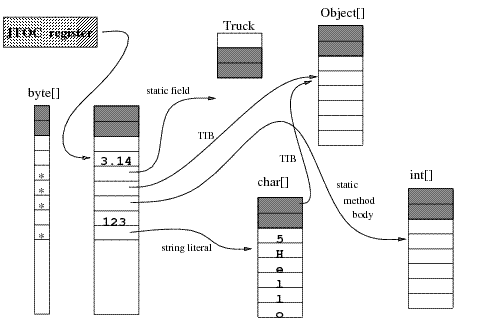
\includegraphics[width=\linewidth]{images/ClassAndCodeManagement-JTOC.png}
\end{figure}

\end{subsubsection}

\begin{subsubsection}{Virtual Methods}

A TIB contains pointers to the compiled method bodies (executable code) for the virtual methods and other instance methods of its class. Thus, the TIB serves as Jikes RVM's virtual method table. A virtual method dispatch entails loading the TIB pointer from the object reference, loading the address of the method body at a given offset off the TIB pointer, and making an indirect branch and link to it. A virtual method is dispatched to with the invokevirtual bytecode; other instance methods are invoked by the invokespecial bytecode.

\end{subsubsection}

\begin{subsubsection}{Static Fields and Methods}

Static fields and pointers to static method bodies are stored in the JTOC. Static method dispatch is simpler than virtual dispatch, since a well-known JTOC entry method holds the address of the compiled method body.

\end{subsubsection}

\begin{subsubsection}{Instance Initialization Methods}

Pointers to the bodies of instance initialization methods, \spverb+<init>+, are stored in the JTOC. (They are always dispatched to with the \spverb+invokespecial+ bytecode.)

\end{subsubsection}

\begin{subsubsection}{Lazy Method Compilation}

Method slots in a TIB or the JTOC may hold either a pointer to the compiled code, or a pointer to the compiled code of the \textit{lazy method invocation stub}. When invoked, the lazy method invocation stub compiles the method, installs a pointer to the compiled code in the appropriate TIB or the JTOC slot, then jumps to the start of the compiled code.

\end{subsubsection}

\begin{subsubsection}{Interface Methods}

Regardless of whether or not a virtual method is overridden, virtual method dispatch is still simple since the method will occupy the same TIB offset its defining class and in every sub-class. However, a method invoked through an \spverb+invokeinterface+ call rather than an \spverb+invokevirtual+ call, will not occupy the same TIB offset in every class that implements its interface. This complicates dispatch for \spverb+invokeinterface+.

The simplest, and least efficient way, of locating an interface method is to search all the virtual method entries in the TIB finding a match. Instead, Jikes RVM uses an \textit{Interface Method Table (IMT)} which resembles a virtual method table for interface methods. Any method that could be an interface method has a fixed offset into the IMT just as with the TIB. However, unlike in the TIB, two different methods may share the same offset into the IMT. In this case, a \textit{conflict resolution stub} is inserted in the IMT. Conflict resolution stubs are custom-generated machine code sequences that test the value of a hidden parameter to dispatch to the desired interface method. For more details, see \spverb+InterfaceInvocation+.

\end{subsubsection}

\end{subsection}

\end{section}


\setNextFileName{ThreadManagement.html}
\begin{section}{Thread Management}
\label{sec:threadmanagement}

This section provides some explanation of how Java\textsuperscript{TM} threads are scheduled and synchronized by Jikes\textsuperscript{TM} RVM.

All Java threads (application threads, garbage collector threads, etc.) derive from \spverb+RVMThread+. Each \spverb+RVMThread+ maps directly to one native thread, which may be implemented using whichever C/C++ threading library is in use (currently pthreads). Unless \spverb+-X:availableProcessors+ or \spverb+-X:gc:threads+ is used, native threads are allowed to be arbitrarily scheduled by the OS using whatever processor resources are available; Jikes\textsuperscript{TM} RVM does not attempt to control the thread-processor mapping at all.

Using native threading gives Jikes\textsuperscript{TM} RVM better compatibility for existing JNI code, as well as improved performance, and greater infrastructure simplicity. Scheduling is offloaded entirely to the operating system; this is both what native code would expect and what maximizes the OS scheduler's ability to optimally schedule Java\textsuperscript{TM} threads. As well, the resulting VM infrastructure is both simpler and more robust, since instead of focusing on scheduling decisions it can take a "hands-off" approach except when Java threads have to be preempted for sampling, on-stack-replacement, garbage collection, \spverb+Thread.suspend()+, or locking. The main task of \spverb+RVMThread+ and other code in \spverb+org.jikesrvm.scheduler+ is thus to override OS scheduling decisions when the VM demands it.

The remainder of this section is organized as follows. The management of a thread's state is discussed in detail. Mechanisms for blocking and handshaking threads are described. The VM's internal locking mechanism, the Monitor, is described. Finally, the locking implementation is discussed.

\begin{subsection}{Tracking the Thread State}

The state of a thread is broken down into two elements:
\begin{itemize}
  \item Should the thread yield at a safe point?
  \item Is the thread running Java code right now?
\end{itemize}

The first mechanism is provided by the \spverb+RVMThread.takeYieldpoint+ field, which is \spverb+0+ if the thread should not yield, or non-zero if it should yield at the next safe point. Negative versus positive values indicate the type of safe point to yield at (epilogue/prologue, or any, respectively).

But this alone is insufficient to manage threads, as it relies on all threads being able to reach a safe point in a timely fashion. New Java threads may be started at any time, including at the exact moment that the garbage collector is starting; a starting-but-not-yet-started thread may not reach a safe point if the thread that was starting it is already blocked. Java threads may terminate at any time; terminated threads will never again reach a safe point. Any Java thread may call into arbitrary JNI code, which is outside of the VM's control, and may run for an arbitrary amount of time without reaching a Java safe point. As well, other mechanisms of \spverb+RVMThread+ may cause a thread to block, thereby making it incapable of reaching a safe point in a timely fashion. However, in each of these cases, the Java thread is "effectively safe" - it is not running Java code that would interfere with the garbage collector, on-stack-replacement, locking, or any other Java runtime mechanism. Thus, a state management system is needed that would notify these runtime services when a thread is "effectively safe" and does not need to be waited on.

RVMThread provides for the following thread states, which describe to other runtime services the state of a Java thread. These states are designed with extreme care to support the following features:
\begin{itemize}
  \item Allow Java threads to either execute Java code, which periodically reaches safe points, and native code which is "effectively safe" by virtue of not having access to VM services.
  \item Allow other threads (either Java threads or VM threads) to asynchronously request a Java thread to block. This overlaps with the takeYieldpoint mechanism, but adds the following feature: a thread that is "effectively safe" does not have to block.
  \item Prevent race conditions on state changes. In particular, if a thread running native code transitions back to running Java code while some other thread expects it to be either "effectively safe" or blocked at a safe point, then it should block. As well, if we are waiting on some Java thread to reach a safe point but it instead escapes into running native code, then we would like to be notified that even though it is not at a safe point, it is now effectively safe, and thus, we do not have to wait for it anymore.
\end{itemize}


The states used to put these features into effect are listed below.
\begin{itemize}
  \item \spverb+NEW+. This means that the thread has been created but is not started, and hence is not yet running. \spverb+NEW+ threads are always effectively safe, provided that they do not transition to any of the other states.
  \item \spverb+IN_JAVA+. The thread is running Java code. This almost always corresponds to the OS "runnable" state - i.e. the thread has no reason to be blocked, is on the runnable queue, and if a processor becomes available it will execute, if it is not already executing. \spverb+IN_JAVA+ thread will periodically reach safe points at which the \spverb+takeYieldpoint+ field will be tested. Hence, setting this field will ensure that the thread will yield in a timely fashion, unless it transitions into one of the other states in the meantime.
  \item \spverb+IN_NATIVE+. The thread is running either native C code, or internal VM code (which, by virtue of Jikes\textsuperscript{TM} RVM's metacircularity, may be written in Java). \spverb+IN_NATIVE+ threads are "effectively safe" in that they will not do anything that interferes with runtime services, at least until they transition into some other state. The \spverb+IN_NATIVE+ state is most often used to denote threads that are blocked, for example on a lock.
  \item \spverb+IN_JNI+. The thread has called into JNI code. This is identical to the \spverb+IN_NATIVE+ state in all ways except one: \spverb+IN_JNI+ threads have a JNIEnvironment that stores more information about the thread's execution state (stack information, etc), while \spverb+IN_NATIVE+ threads save only the minimum set of information required for the GC to perform stack scanning.
  \item \spverb+IN_JAVA_TO_BLOCK+. This represents a thread that is running Java code, as in \spverb+IN_JAVA+, but has been requested to yield. In most cases, when you set \spverb+takeYieldpoint+ to non-zero, you will also change the state of the thread from \spverb+IN_JAVA+ to \spverb+IN_JAVA_TO_BLOCK+. If you don't intend on waiting for the thread (for example, in the case of sampling, where you're opportunistically requesting a yield), then this step may be omitted; but in the cases of locking and garbage collection, when a thread is requested to yield using \spverb+takeYieldpoint+, its state will also be changed.
  \item \spverb+BLOCKED_IN_NATIVE+. \spverb+BLOCKED_IN_NATIVE+ is to \spverb+IN_NATIVE+ as \newline \spverb+IN_JAVA_TO_BLOCK+ is to \spverb+IN_JAVA+. When requesting a thread to yield, we check its state; if it's \spverb+IN_NATIVE+, we set it to be \spverb+BLOCKED_IN_NATIVE+.
  \item \spverb+BLOCKED_IN_JNI+. Same as \spverb+BLOCKED_IN_NATIVE+, but for \spverb+IN_JNI+.
  \item \spverb+TERMINATED+. The thread has died. It is "effectively safe", but will never again reach a safe point.
\end{itemize}

The states are stored in \spverb+RVMThread.execStatus+, an integer field that may be rapidly manipulated using compare-and-swap. This field uses a hybrid synchronization protocol, which includes both compare-and-swap and conventional locking (using the thread's Monitor, accessible via the \spverb+RVMThread.monitor()+ method). The rules are as follows:

\begin{itemize}
  \item All state changes except for \spverb+IN_JAVA+ to \spverb+IN_NATIVE+ or \spverb+IN_JNI+, and \newline \spverb+IN_NATIVE+ or \spverb+IN_JNI+ back to \spverb+IN_JAVA+, must be done while holding the lock.
  \item Only the thread itself can change its own state without holding the lock.
  \item The only asynchronous state changes (changes to the state not done by the thread that owns it) that are allowed are \spverb+IN_JAVA+ to \spverb+IN_JAVA_TO_BLOCK+, \spverb+IN_NATIVE+ to \spverb+BLOCKED_IN_NATIVE+, and \spverb+IN_JNI+ TO \spverb+BLOCKED_IN_JNI+.
\end{itemize}

The typical algorithm for requesting a thread to block looks as follows:

\begin{lstlisting}[language=Java]
thread.monitor().lockNoHandshake();
if (thread is running) {
   thread.takeYieldpoint=1;

   // transitions IN_JAVA -> IN_JAVA_TO_BLOCK, IN_NATIVE->BLOCKED_IN_NATIVE, etc.
   thread.setBlockedExecStatus(); 
   
   if (thread.isInJava()) {
      // Thread will reach safe point soon, or else notify 
      // us that it left to native code.
      // In either case, since we are holding the lock, 
      // the thread will effectively block on either the safe point
      // or on the attempt to go to native code, since performing
      // either state transition requires acquiring the lock,
      // which we are now holding.
   } else {
      // Thread is in native code, and thus is "effectively safe",
      // and cannot go back to running Java code so long as we hold
      // the lock, since that state transition requires
      // acquiring the lock.
   }
}
thread.monitor().unlock();
\end{lstlisting}

Most of the time, you do not have to write such code, as the cases of blocking threads are already implemented. For examples of how to utilize these mechanisms, see \texttt{RVM\-Thread.block()}, \texttt{RVM\-Thread.hard\-Hand\-sha\-ke\-Sus\-pend()}, and \texttt{RVM\-Thread.soft\-Hand\-sha\-ke()}. A discussion of how to use these methods follows in the section below.

Finally, the valid state transitions are as follows.
\begin{itemize}
  \item \spverb+NEW+ to \spverb+IN_JAVA+: occurs when the thread is actually started. At this point it is safe to expect that the thread will reach a safe point in some bounded amount of time, at which point it will have a complete execution context, and this will be able to have its stack traces by GC.
  \item \spverb+IN_JAVA+ to \spverb+IN_JAVA_TO_BLOCK+: occurs when an asynchronous request is made, for example to stop for GC, do a mutator flush, or do an isync on PPC.
  \item \spverb+IN_JAVA+ to \spverb+IN_NATIVE+: occurs when the code opts to run in privileged mode, without synchronizing with GC. This state transition is only performed by Monitor, in cases where the thread is about to go idle while waiting for notifications (such as in the case of park, wait, or sleep), and by org.jikesrvm.runtime.FileSystem, as an optimization to allow I/O operations to be performed without a full JNI transition.
  \item \spverb+IN_JAVA+ to \spverb+IN_JNI+: occurs in response to a JNI downcall, or return from a JNI upcall.
  \item \spverb+IN_JAVA_TO_BLOCK+ to \spverb+BLOCKED_IN_NATIVE+: occurs when a thread that had been asked to perform an async activity decides to go to privileged mode instead. This state always corresponds to a notification being sent to other threads, letting them know that this thread is idle. When the thread is idle, any asynchronous requests (such as mutator flushes) can instead be performed on behalf of this thread by other threads, since this thread is guaranteed not to be running any user Java code, and will not be able to return to running Java code without first blocking, and waiting to be unblocked (see \spverb+BLOCKED_IN_NATIVE+ to \spverb+IN_JAVA+ transition.
  \item \spverb+IN_JAVA_TO_BLOCK+ to \spverb+BLOCKED_IN_JNI+: occurs when a thread that had been asked to perform an async activity decides to make a JNI downcall, or return from a JNI upcall, instead. In all other regards, this is identical to the \spverb+IN_JAVA_TO_BLOCK+ to \spverb+BLOCKED_IN_NATIVE+ transition.
  \item \spverb+IN_NATIVE+ to \spverb+IN_JAVA+: occurs when a thread returns from idling or running privileged code to running Java code.
  \item \spverb+BLOCKED_IN_NATIVE+ to \spverb+IN_JAVA+: occurs when a thread that had been asked to perform an async activity while running privileged code or idling decides to go back to running Java code. The actual transition is preceded by the thread first performing any requested actions (such as mutator flushes) and waiting for a notification that it is safe to continue running (for example, the thread may wait until GC is finished).
  \item \spverb+IN_JNI+ to \spverb+IN_JAVA+: occurs when a thread returns from a JNI downcall, or makes a JNI upcall.
  \item \spverb+BLOCKED_IN_JNI+ to \spverb+IN_JAVA+: same as \spverb+BLOCKED_IN_NATIVE+ to \spverb+IN_JAVA+, except that this occurs in response to a return from a JNI downcall, or as the thread makes a JNI upcall.
  \item \spverb+IN_JAVA+ to \spverb+TERMINATED+: the thread has terminated, and will never reach any more safe points, and thus will not be able to respond to any more requests for async activities.
\end{itemize}

\end{subsection}

\begin{subsection}{Blocking and Handshaking}

Various VM services, such as the garbage collector and locking, may wish to request a thread to block. In some cases, we want to block all threads except for the thread that makes the request. As well, some VM services may only wish for a "soft handshake", where we wait for each non-collector thread to perform some action exactly once and then continue (in this case, the only thread that blocks is the thread requesting the soft handshake, but all other non-collector threads must "yield" in order to perform the requested action; in most cases that action is non-blocking). A unified facility for performing all of these requests is provided by \spverb+RVMThread+.

Four types of thread blocking and handshaking are supported:
\begin{itemize}
  \item \spverb+RVMThread.block()+. This is a low-level facility for requesting that a particular thread blocks. It is inherently unsafe to use this facility directly - for example, if thread \spverb+A+ calls \spverb+B.block()+ while thread \spverb+B+ calls \spverb+A.block()+, the two threads may mutually deadlock.
  \item \spverb+RVMThread.beginPairHandshake()+. This implements a safe pair\hyp handshaking mechanism, in which two threads become bound to each other for a short time. The thread requesting the pair handshake waits until the other thread is at a safe point or else is "effectively safe", and prevents it from going back to executing Java code. Note that at this point, neither thread will respond to any other handshake requests until \texttt{RVM\-Thread.end\-Pair\-Hand\-sha\-ke()} is called. This is useful for implementing biased locking, but it has general utility anytime one thread needs to manipulate something another thread's execution state.
  \item \spverb+RVMThread.softHandshake()+. This implements soft handshakes. In a soft handshake, the requesting thread waits for all non-collector threads to perform some action exactly once, and then returns. If any of those threads are effectively safe, then the requesting thread performs the action on their behalf. \spverb+softHandshake()+ is invoked with a \texttt{Soft\-Hand\-sha\-ke\-Vi\-si\-tor} that determines which threads are to be affected, and what the requested action is. An example of how this is used is found in \texttt{org.ji\-kes\-rvm.mm.mmtk.Col\-lec\-tion} and \texttt{org.ji\-kes\-rvm.com\-pi\-lers.opt.run\-ti\-me\-sup\-port.Opt\-Com\-pi\-led\-Me\-thod}.
  \item \spverb+RVMThread.hardHandshakeSuspend()+. This stops all threads except for the garbage collector threads and the thread making the request. It returns once all Java threads are stopped. This is used by the garbage collector itself, but may be of utility elsewhere (for example, dynamic software updating). To resume all stopped threads, call \texttt{RVM\-Thread.hard\-Hand\-sha\-ke\-Re\-su\-me()}. Note that this mechanism is carefully designed so that even after the world is stopped, it is safe to request a garbage collection (in that case, the garbage collector will itself call a variant of \texttt{hard\-Hand\-sha\-ke\-Sus\-pend()}, but it will only affect the one remaining running Java thread).
\end{itemize}

\end{subsection}

\begin{subsection}{The Monitor API}

The VM internally uses an OS-based locking implementation, augmented with support for safe lock recursion and awareness of handshakes. The Monitor API provides locking and notification, similar to a Java lock, and is implemented using a \spverb+pthread_mutex+ and a \spverb+pthread_cond+.

Acquiring a Monitor lock, or awaiting notification, may cause the calling \texttt{RVM\-Thread} to block. This prevents the calling thread from acknowledging handshakes until the blocking call returns. In some cases, this is desirable. For example:
\begin{itemize}
  \item In the implementation of handshakes, the code already takes special care to use the \texttt{RVM\-Thread} state machine to notify other threads that the caller may block. As such, acquiring a lock or waiting for a notification is safe.
  \item If acquiring a lock that may only be held for a short, guaranteed-bounded length of time, the fact that the thread will ignore handshake requests while blocking is safe - the lock acquisition request will return in bounded time, allowing the thread to acknowledge any pending handshake requests.
\end{itemize}

But in all other cases, the calling thread must ensure that the handshake mechanism is notified that thread will block. Hence, all blocking \spverb+Monitor+ methods have both a "NoHandshake" and "WithHandshake" version. Consider the following code:

\begin{lstlisting}[language=Java]
someMonitor.lockNoHandshake();
// perform fast, bounded-time critical section
someMonitor.unlock(); // non-blocking
\end{lstlisting}

In this code, lock acquisition is done without notifying handshakes. This makes the acquisition faster. In this case, it is safe because the critical section is bounded-time. As well, we require that in this case, any other critical sections protected by \spverb+someMonitor+ are bounded-time as well. If, on the other hand, the critical section was not bounded-time, we would do:

\begin{lstlisting}[language=Java]
someMonitor.lockWithHandshake();
// perform potentially long critical section
someMonitor.unlock();
\end{lstlisting}

In this case, the \spverb+lockWithHandshake()+ operation will transition the calling thread to the \spverb+IN_NATIVE+ state before acquiring the lock, and then transition it back to \spverb+IN_JAVA+ once the lock is acquired. This may cause the thread to block, if a handshake is in progress. As an added safety provision, if the \spverb+lockWithHandshake()+ operation blocks due to a handshake, it will ensure that it does so without holding the \spverb+someMonitor+ lock.

A special \spverb+Monitor+ is provided with each thread. This monitor is of the type \texttt{No\-Yield\-points\-Mo\-ni\-tor} and will also ensure that yieldpoints (safe points) are disabled while the lock is held. This is necessary because any safe point may release the \texttt{Monitor} lock by waiting on it, thereby breaking atomicity of the critical section. The \texttt{No\-Yield\-points\-Mo\-ni\-tor} for any \texttt{RVM\-Thread} may be accessed using the \texttt{RVM\-Thread.mo\-ni\-tor()} method.

Additional information about how to use this API is found in the following section, which discusses the implementation of Java locking.

\end{subsection}

\begin{subsection}{Thin and Biased Locking}

Jikes\textsuperscript{TM} RVM uses a hybrid thin/biased locking implementation that is designed for very high performance under any of the following loads:
\begin{itemize}
  \item Locks only ever acquired by one thread. In this case, biased locking is used, an no atomic operations (like compare-and-swap) need to be used to acquire and release locks.
  \item Locks acquired by multiple threads but rarely under contention. In this case, thin locking is used; acquiring and releasing the lock involves a fast inlined compare-and-swap operation. It is not as fast as biased locking on most architectures.
  \item Contended locks. Under sustained contention, the lock is "inflated" - the lock will now consist of data structures used to implement a fast barging FIFO mutex. A barging FIFO mutex allows threads to immediately acquire the lock as soon as it is available, or otherwise enqueue themselves on a FIFO and await its availability.
\end{itemize}

Thin locking has a relatively simple implementation; roughly 20 bits in the object header are used to represent the current lock state, and compare-and-swap is used to manipulate it. Biased locking and contended locking are more complicated, and are described below.

Biased locking makes the optimistic assumption that only one thread will ever want to acquire the lock. So long as this assumption holds, acquisition of the lock is a simple non-atomic increment/decrement. However, if the assumption is violated (a thread other than the one to which the lock is biased attempts to acquire the lock), a fallback mechanism is used to turn the lock into either a thin or contended lock. This works by using \texttt{RVM\-Thread.be\-gin\-Pair\-Hand\-sha\-ke()} to bring both the thread that is requesting the lock and the thread to which the lock is biased to a safe point. No other threads are affected; hence this system is very scalable. Once the pair handshake begins, the thread requesting the lock changes the lock into either a thin or contended lock, and then ends the pair handshake, allowing the thread to which the lock was biased to resume execution, while the thread requesting the lock may now contend on it using normal thin/contended mechanisms.

Contended locks, or "fat locks", consist of three mechanisms:
\begin{enumerate}
  \item A spin lock to protect the data structures.
  \item  A queue of threads blocked on the lock.
  \item  A mechanism for blocked threads to go to sleep until awoken by being dequeued.
\end{enumerate}

The spin lock is a \spverb+org.jikesrvm.scheduler.SpinLock+. The queue is implemented in \texttt{org.jikes\-rvm.sche\-du\-ler.Thread\-Queue}. And the blocking/unblocking mechanism leverages \texttt{org.jikes\-rvm.sche\-du\-ler.Mo\-ni\-tor}; in particular, it uses the \spverb+Monitor+ that is attached to each thread, accessible via \texttt{RVM\-Thread.mo\-ni\-tor()}. The basic algorithm for lock acquisition is:
\begin{lstlisting}[language=Java]
spinLock.lock();
while (true) {
   if (lock available) {
      acquire the lock;
      break;
   } else {
      queue.enqueue(me);
      spinLock.unlock();

      me.monitor().lockNoHandshake();
      while (queue.isQueued(me)) {
         // put this thread to sleep waiting to be dequeued, 
         // and do so while the thread is IN_NATIVE to ensure 
         // that other threads don't wait on this one for
         // handshakes while we're blocked.
         me.monitor().waitWithHandshake();
      }
      me.monitor().unlock();
      spinLock.lock();
   }
}
spinLock.unlock();
\end{lstlisting}

The algorithm for unlocking dequeues the thread at the head of the queue (if there is one) and notifies its \spverb+Monitor+ using the \texttt{locked\-Broad\-cast\-No\-Hand\-sha\-ke()} method. Note that these algorithms span multiple methods in \texttt{org.jikes\-rvm.sche\-du\-ler.Thin\-Lock} and \texttt{org.jikes\-rvm.sche\-du\-ler.Lock}; in particular, \texttt{lock\-Heavy()}, \texttt{lock\-Hea\-vy\-Locked()}, \texttt{un\-lock\-Hea\-vy()}, \texttt{lock()}, and \texttt{un\-lock()}.

\end{subsection}

\end{section}


\setNextFileName{JNI.html}
\begin{section}{JNI}
\label{sec:jni}

\begin{subsection}{Overview}

This section describes how Jikes RVM interfaces to native code. There are three major aspects of this support:
\begin{itemize}
  \item JNI Functions: This is the mechanism for transitioning from native code into Java code. Jikes RVM implements the 1.1 through 1.4 JNI specifications.
  \item Native methods: This is the mechanism for transitioning from Java code to native code. In addition to the normal mechanism used to invoke a native method, Jikes RVM also supports a more restricted syscall mechanism that is used internally by low-level VM code to invoke native code.
  \item Integration with threading: JNI may be freely used from any Java method. The mechanisms required to make this work are discussed in great detail in \hyperref[sec:threadmanagement]{Thread Management}, and to some extent in the sections that follow.
\end{itemize}

\end{subsection}

\begin{subsection}{JNI Functions}

All of the 1.1 through 1.4 JNIEnv interface functions are implemented.

The functions are defined in the class \texttt{JNI\-Func\-tions}. Methods of this class are compiled with special prologues/epilogues that translate from native calling conventions to Java calling conventions and handle other details of the transition related to threading. Currently the optimizing compiler does not support these specialized prologue/epilogue sequences so all methods in this class are baseline compiled. The prologue/epilogue sequences are actually generated by the platform-specific \texttt{JNI\-Com\-pi\-ler}.

Calling a JNI function results in the thread attempting to transition from \spverb+IN_JNI+ to \spverb+IN_JAVA+ using a compare-and-swap; if this fails, the thread may block to acknowledge a handshake. See \hyperref[sec:threadmanagement]{Thread Management} for more details.

\end{subsection}

\begin{subsection}{Invoking Native Methods}

There are two mechanisms whereby RVM may transition from Java code to native code.

The first mechanism is when RVM calls a method of the class \texttt{SysCall}. The native methods thus invoked are defined in one of the C and C++ files of the JikesRVM executable. These native methods are non-blocking system calls or C library services. To implement a syscall, Jikes RVM compilers generate a call sequence consistent with the platform's underlying calling convention. A syscall is not a GC-safe point, so syscalls may modify the Java heap (eg. \spverb+memcpy()+). For more details on the mechanics of adding a new syscall to the system, see the header comments of \texttt{Sys\-Call.java}. Note again that the syscall methods are NOT JNI methods, but an independent (more efficient) interface that is specific to Jikes RVM.

The second mechanism is JNI. Naturally, the user writes JNI code using the JNI interface. RVM implements a call to a native method by using the platform-specific \texttt{JNI\-Com\-pi\-ler} to generate a stub routine that manages the transition between Java bytecode and native code. A JNI call is a GC-safe point, since JNI code cannot freely modify the Java heap.

\end{subsection}

\begin{subsection}{Interactions with Threading}

See the \hyperref[sec:threadmanagement]{Thread Management} subsection for more details on the thread system in Jikes RVM.

There are two ways to execute native code: syscalls and JNI. A Java thread that calls native code by either mechanism will never be preempted by Jikes RVM, but in the case of JNI, all of the VM's services will know that the thread is "effectively safe" and thus may be ignored for most purposes. Additionally, threads executing JNI code may have handshake actions performed by other threads on their behalf, for example in the case of GC stack scanning. This is not the case with syscalls. As far as Jikes RVM is concerned, a Java thread that enters syscall native code is still executing Java code, but will appear to not reach a safe point until after it emerges from the syscall. This issue may be side-stepped by using the \texttt{RVM\-Thread} \texttt{en\-ter\-Na\-ti\-ve()} and \texttt{lea\-ve\-Na\-ti\-ve} methods, as shown in \texttt{org.jikes\-rvm.run\-ti\-me.Fi\-le\-Sys\-tem}.

\end{subsection}

\begin{subsection}{Missing Features}

\begin{itemize}
  \item \textbf{Native Libraries:} JNI 1.2 requires that the VM specially treat native libraries that contain exported functions named \spverb+JNI_OnLoad+ and \newline \spverb+JNI_OnUnload+. Only \spverb+JNI_OnLoad+ is currently implemented.
  \item \textbf{\texttt{JNI\-Com\-pi\-ler}:} The only known deficiency in \texttt{JNI\-Com\-pi\-ler} is that the prologue and epilogues only handle passing local references to functions that expect a \spverb+jobject+; they will not properly handle a \spverb+jweak+ or a regular global reference. This would be fairly easy to implement.
  \item \textbf{JavaVM interface:} The JavaVM interface has \spverb+GetEnv+ fully implemented and \texttt{AttachCurrentThread} partly implemented, but \texttt{DestroyJavaVM}, \texttt{DetachCurrentThread}, and \texttt{AttachCurrentThreadAsDaemon} are just stubbed out and return error codes. There is no good reason why \texttt{AttachCurrentThread} and friends cannot be implemented; it just hasn't been done yet, mostly because there was no easy way to support them prior to the introduction of native threads.
  \item \textbf{Directly-Exported Invocation Interface Functions:} These functions (\texttt{Get\-De\-fault\-Ja\-va\-VM\-Init\-Args} and \texttt{JNI\_Cre\-ate\-Ja\-va\-VM} are partly implemented but \texttt{JNI\_Get\-Crea\-ted\-Ja\-va\-VMs}) is not implemented. This is because we do not provide a virtual machine library that can be linked against, nor do we support native applications that launch and use an embedded Java VM. There is no inherent reason why this could not be done, but we have not done so yet.
\end{itemize}

\end{subsection}

\begin{subsection}{Things JNI Can't Handle}

\begin{itemize}
  \item \textbf{atexit routines:} Calling JNI code via a routine run at exit time means calling back into a VM that has been shutdown. This will cause the Jikes RVM to freeze on Intel architectures.
\end{itemize}

Contributions of any of the missing functionality (and/or associated tests) would be greatly appreciated.

\end{subsection}

\end{section}


\setNextFileName{Exception Management.html}
\begin{section}{Exception Management}
\label{sec:exceptionmanagement}

The runtime has to deal with the relatively small number of hardware signals which can be generated during Java execution. On operating systems other than AIX, an attempt to dereference a \spverb+null+ value (an access to a null value manifests as a read to a small negative address outside the mapped virtual memory address space) will generate a a segmentation fault. This means that the Jikes RVM does not need to generate explicit tests guarding against dereferencing null values and this results in faster code generationg for non-excepting code.

The Jikes RVM handles the signal and reenters Java so that a suitable Java exception handler can be identified, the stack can be unwound (if necessary) and the handler entered in order to deal with the exception. Failing location of a handler, the associated Java thread must be cleanly terminated.

The Jikes RVM actually employs software traps to generate hardware exceptions in a small number of other cases, for example to trap array bounds exceptions. Once again a software only solution would be feasible. However, since a mechanism is already in place to catch hardware exceptions and restore control to a suitable Java handler the use of software traps is relatively simple to support.

Use of a hardware handler enables the register state at the point of exception to be saved by the hardware exception catching routine. If a Java handler is registered in the call frame which generated the exception this register state can be restored before reentry, avoiding the need for the compiler to save register state around potentially excepting instructions. Register state for handlers in frames below the exception frame is automatically saved by the compiler before making a call and so can always be restored to the state at the point of call by the exception delivery code.

The bootloader registers signal handlers which catch \spverb+SEGV+ and \spverb+TRAP+ signals. These handlers save the current register state on the stack, create a special handler frame above the saved register state and return into this handler frame executing \texttt{Run\-ti\-me\-En\-try\-points.de\-li\-ver\-Hard\-wa\-re\-Ex\-cep\-tion()}. This method searches the stack from the excepting frame (or from the last Java frame if the exception occurs inside native code) looking for a suitable handler and unwinding frames which do not contain one. At each unwind the saved register state is reset to the state associated with the next frame. When a handler is found the delivery code installs the saved register state and returns into the handler frame at the start of the handler block.

The Jikes RVM employs some of the same code used by the hardware exception handler to implement the language primitive \spverb+throw()+. This primitive requires a handler to be located and the stack to be unwound so that the handler can be entered. A \spverb+throw+ operation is always translated into a call to \texttt{Run\-ti\-me\-En\-try\-points.a\-throw()} so the unwind can never happens in the handler frame. Hence the register state at the point of re-entry is always saved by the call mechanism and there is no need to generate a hardware exception.

\end{section}


\setNextFileName{Bootstrap.html}
\begin{section}{Bootstrap}
\label{sec:bootstrap}

Jikes RVM is started up by a boot program written in C, the bootloader. The bootloader is responsible for
\begin{itemize}
  \item registering signal handlers to deal with the hardware errors generated by the RVM
  \item establishing the initial virtual memory map employed by Jikes RVM
  \item mapping the Jikes RVM image files
  \item installing the addresses of the C wrapper functions which are invoked by the runtime to interact with the underlying operating system into the boot record of at the start of the RVM image area
  \item setting up the JTOC and TR registers for its RVMThread/pthread
  \item switching the pthread into the bootstrap Java stack running the bootstrap Java method in the bootstrap Java thread
\end{itemize}

At this point all further initialization of the RVM is done either in Java or by employing the wrapper callbacks located in the boot record.

The initial bootstrap routine is \spverb+VM.boot()+. It sets up the initial thread environment so that it looks like any other thread created by a call to \spverb+Thread.start()+ then performs a variety of Java boot operations, including initialising the memory manager subsystem, the runtime compiler, the system classloader and the time classes.

The bootstrap routine needs to rerun class initializers for a variety of the runtime and runtime library classes which are already loaded and compiled into the image file. This is necessary because some of the data generated by these initialization routines will not be valid in the JIkes RVM runtime. The data may be invalid as the host environment that generated the boot image may differ from the current environment.

The boot process the enables the Java scheduler and locking system, setting up the data structures necessary to launch additional threads. The scheduler also starts the \texttt{Fi\-na\-li\-zer\-Thread} and multiple garbage collector threads (i.e. multiple instances of \texttt{Col\-lec\-tor\-Thread}).

Next, the boot routine boots the the JNI subsystem which enables calls to native code to be compiled and executed then re-initialises a few more classes whose init methods require a functional JNI (i.e. \texttt{ja\-va.io.Fi\-le\-Des\-crip\-tor}).

Finally, the boot routine loads the boot application class supplied on the rvm command line, creates and schedules a Java main thread to execute this class's main method, then exits, switching execution to the main thread. Execution continues until the application thread and all non-daemon threads have exited. Once there are no runnable threads (other than system threads such as the idle threads, collector threads etc) execution of the RVM runtime terminates and the rvm process exits.

\begin{subsection}{Memory Map}

The RVM divides its available virtual memory space into various segments containing either code, or data or a combination of the two. The basic map is as follows:
% For basicstyle:
%   \small (the current default) is much too large, and \footnotesize is slightly too large. \tiny is too small.
%   \ttfamily is necessary so that the map looks like it did in the old user guide
\begin{lstlisting}[basicstyle=\scriptsize\ttfamily,frame=none] 

                   +--> BOOT_IMAGE_START   MAX_MAPPABLE_ADDRESS <--+
                   |<- SEGMENT_SIZE ->                             |
+-------------------------------------------------------------------------+
+ Platform specific| RVM Image       | RVM Heap                    | Plat +
+ ( booter code/ ) | ( initial code )| ( meta data, immortal data )| spec +
+ ( data, shlibs ) | (  & data      )| ( large & small objects    )|      +
+-------------------------------------------------------------------------+
\end{lstlisting}

\begin{subsubsection}{Boot Segment}

The bottom segment of the address space is left for the underlying platform to locate the boot program (including statically linked library code) and any dynamically allocated data and library code.

\end{subsubsection}

\begin{subsubsection}{RVM Image Segment}

The next area is the one initialized by the boot program to contain the all the initial static data, instance data and compiled method code required in order for the runtime to be able to function. The required memory data is loaded from an image file created by an off line Java program, the boot image writer.

This image file is carefully constructed to contain data which, when loaded at the correct address, will populate the runtime data area with a memory image containing:

\begin{itemize}
  \item a JTOC
  \item all the TIBs, static method code arrays and static field data directly referenced from the JTOC
  \item all the dynamic method code arrays indirectly referenced from the TIBS
  \item all the classloader's internal class and method instances indirectly referenced via the TIBS
  \item ancillary structures attached to these class and method instances such as class bytecode arrays, compilation records, garbage collection maps etc
  \item a single bootstrap Java thread instance in which Java execution commences
  \item a single bootstrap thread stack used by the bootstrap thread.
  \item a master boot record located at the start of the image load area containing references to all the other key objects in the image (such as the JTOC, the bootstrap thread etc) plus linkage slots in which the booter writes the addresses of its C callback functions.
\end{itemize}

\end{subsubsection}

\begin{subsubsection}{RVM Heap Segment}

The RVM heap segment is used to provide storage for code and data created during Java execution. The RVM can be configured to employ various different allocation managers taken from the MMTk memory management toolkit.

\end{subsubsection}

\end{subsection}

\end{section}


\setNextFileName{CallingConventions.html}
\begin{section}{Calling Conventions}
\label{sec:callingconventions}

\begin{subsection}{Architecture-independent concepts}

Stackframe layout and calling conventions may evolve as our understanding of Jikes RVM's performance improves. Where possible, API's should be used to protect code against such changes.

\begin{subsubsection}{Register conventions}

Registers (general purpose, gp, and floating point, fp) can be roughly categorized into four types:
\begin{itemize}
  \item \textbf{Scratch:} Needed for method prologue/epilogue. Can be used by compiler between calls.
  \item \textbf{Dedicated:} Reserved registers with known contents:
    \begin{itemize}
      \item \textbf{JTOC} - Jikes RVM Table Of Contents. Globally accessible data: constants, static fields and methods.
      \item \textbf{FP} - Frame Pointer Current stack frame (thread specific).
      \item \textbf{TR} - Thread register. An object representing the current \spverb+RVMThread+ instance (the one executing on the CPU containing these registers).
    \end{itemize}
  \item \textbf{Volatile ("caller save", or "parameter"):} Like scratch registers, these can be used by the compiler as temporaries, but they are not preserved across calls. Volatile registers differ from scratch registers in that volatiles can be used to pass parameters and result(s) to and from methods.
  \item \textbf{Nonvolatile ("callee save", or "preserved"):} These can be used (and are preserved across calls), but they must be saved on method entry and restored at method exit. Highest numbered registers are to be used first. (At least initially, nonvolatile registers will not be used to pass parameters.)
\end{itemize}

\end{subsubsection}

\begin{subsubsection}{Stack conventions}

Stacks grow from high memory to low memory.

\end{subsubsection}

\begin{subsubsection}{Method prologue responsibilities}

(some of these can be omitted for leaf methods):
\begin{enumerate}
  \item Execute a stackoverflow check, and grow the thread stack if necessary.
  \item Save the caller's next instruction pointer (callee's return address)
  \item Save any nonvolatile floating-point registers used by callee.
  \item Save any nonvolatile general-purpose registers used by callee.
  \item Store and update the frame pointer FP.
  \item Store callee's compiled method ID
  \item Check to see if the Java\textsuperscript{TM} thread must yield the Processor (and yield if threadswitch was requested).
\end{enumerate}

\end{subsubsection}

\begin{subsubsection}{Method epilogue responsibilities}

(some of these can be ommitted for leaf methods):
\begin{enumerate}
  \item Restore FP to point to caller's stack frame.
  \item Restore any nonvolatile general-purpose registers used by callee.
  \item Restore any nonvolatile floating-point registers used by callee.
  \item Branch to the return address in caller.
\end{enumerate}

\end{subsubsection}

\end{subsection}

\begin{subsection}{Architecture-specific calling conventions}

The following architecture-specific classes are of interest for calling conventions:
\begin{itemize}
  \item \spverb+StackframeLayoutConstants+ for layout of the stack frame
  \item \spverb+JNICompiler+ for transition to native code
  \item \spverb+RegisterConstants+ for register definitions
  \item \spverb+BaselineConstants+ for register usage by the baseline compiler
  \item \spverb+CallingConventions+ which expands the calling conventions shortly before register allocation in the optimizing compiler
\end{itemize}

\end{subsection}

\end{section}


\setNextFileName{VMCallbacks.html}
\begin{section}{VM Callbacks}
\label{sec:vmcallbacks}

Jikes\textsuperscript{TM} RVM provides callbacks for many runtime events of interest to the Jikes RVM programmer, such as classloading, VM boot image creation, and VM exit. The callbacks allow arbitrary code to be executed on any of the supported events.

The callbacks are accessed through the nested interfaces defined in the \spverb+Callbacks+ class. There is one interface per event type. To be notified of an event, register an instance of a class that implements the corresponding interface with \spverb+Callbacks+ by calling the corresponding \spverb+add...()+ method. For example, to be notified when a class is instantiated, first implement the \texttt{Call\-backs.Class\-In\-stan\-tia\-ted\-Mo\-ni\-tor} interface, and then call \texttt{Call\-backs.add\-Class\-In\-stan\-tia\-ted\-Mo\-ni\-tor()} with an instance of your class. When any class is instantiated, the \texttt{no\-ti\-fy\-Class\-In\-stan\-tia\-ted} method in your instance will be invoked.

The appropriate interface names can be obtained by appending "Monitor" to the event names (e.g. the interface to implement for the MethodOverride event is \texttt{Call\-backs.Me\-thod\-Over\-ri\-de\-Mo\-ni\-tor}). Likewise, the method to register the callback is "add", followed by the name of the interface (e.g. the register method for the above interface is \texttt{Call\-backs.add\-Me\-thod\-Over\-ri\-de\-Mo\-ni\-tor()}).

Since the events for which callbacks are available are internal to the VM, there are limitations on the behavior of the callback code. For example, as soon as the exit callback is invoked, all threads are considered daemon threads (i.e. the VM will not wait for any new threads created in the callbacks to complete before exiting). Thus, if the exit callback creates any threads, it has to join() with them before returning. These limitations may also produce some unexpected behavior. For example, while there is an elementary safeguard on any classloading callback that prevents recursive invocation (i.e. if the callback code itself causes classloading), there is no such safeguard across events, so, if there are callbacks registered for both ClassLoaded and ClassInstantiated events, and the ClassInstantiated callback code causes dynamic class loading, the ClassLoaded callback will be invoked for the new class, but not the ClassInstantiated callback.

Examples of callback use can be seen in the \spverb+Controller+ class in the adaptive system.

\begin{subsection}{An Example: Modifying SPECjvm98 to Report the End of a Run}

The SPECjvm\textregistered 98 benchmark suite is configured to run one or more benchmarks a particular number of times. For example, the following runs the compress benchmark for 5 iterations:
\begin{lstlisting}
rvm SpecApplication -m5 -M5 -s100 -a _201_compress
\end{lstlisting}

It is sometimes useful to have the VM notified when the application has completed an iteration of the benchmark. This can be performed by using the Callbacks interface. The specifics are specified below:
\begin{enumerate}
  \item Modify \spverb+spec/harness/ProgramRunner.java+:
    \begin{enumerate}
      \item add an import statement for the \spverb+Callbacks+ class:
        \begin{lstlisting}[language=Java]
import org.jikesrvm.Callbacks;
        \end{lstlisting}
      \item before the call to \spverb+runOnce+ add the following:
        \begin{lstlisting}[language=Java]
Callbacks.notifyAppRunStart(className, run);
        \end{lstlisting}
      \item after the call to runOnce add the following:
        \begin{lstlisting}[language=Java]
Callbacks.notifyAppRunComplete(className, run);
        \end{lstlisting}
    \end{enumerate}
  \item Recompile the modified file:
    \begin{lstlisting}
javac -classpath .:$RVM_BUILD/RVM.classes:$RVM_BUILD/RVM.classes/rvmrt.jar spec/harness/ProgramRunner.java
    \end{lstlisting}
    or create a stub version of Callbacks.java and place it the appropriate directory structure with your modified file, i.e., \newline \texttt{org/jikes\-rvm/Call\-backs.java}
  \item  Run Jikes RVM as you normally would using the SPECjvm98 benchmarks.
\end{enumerate}

In the current system the \spverb+Controller+ class will gain control when these callbacks are made and print a message into the AOS log file (by default, placed in Jikes RVM's current working directory and called \spverb+AOSLog.txt+).

\end{subsection}

\begin{subsection}{Another Example: Directing a Recompilation of All Methods During the Application's Execution}

Another callback of interest allows an application to direct the VM to recompile all executed methods at a certain point of the application's execution by calling the \texttt{re\-com\-pi\-le\-All\-Dy\-na\-mi\-cal\-ly\-Loa\-ded\-Me\-thods} method in the \spverb+Callbacks+ class. This functionality can be useful to experiment with the performance effects of when compilation occurs. This VM functionality can be disabled using the \texttt{DIS\-ABLE\_RE\-COM\-PI\-LE\_ALL\_ME\-THODS} boolean flag to the adaptive system.

\end{subsection}

\end{section}



\end{chapter}
